\documentclass[]{tufte-handout}
\usepackage{amsmath, amssymb, amsthm}
\usepackage{hyperref}
\usepackage{framed}
\usepackage[pdftex]{graphicx}
\hypersetup{colorlinks}

\title{COMP161 - Lab 7 \& Homework 5}
\author{}
\date{Spring 2015}

\begin{document}
\maketitle

\begin{abstract}
For this lab you'll work on writing a mutator procedure. For homework you'll work on an output procedure. Both topics are covered in lecture notes 9. 
\end{abstract}

\section{Lab 7}

\begin{framed}
\begin{quote}
An $n$-gram letter frequency analysis counts the frequency of $n$ letter sequences in a string. These statistics can then be used for several purposes in natural language processing and cryptography. A common technique to handle the begging and end of a document is to pad both with $(n-1)$ special characters such that the first $n$ gram is the first letter of the text preceded by $(n-1)	$ special characters and the last $n$ gram is the last character followed by $(n-1)$ special characters. It is usually important that the padding character is unique and doesn't occur elsewhere in the text as it signifies the beginning and end of the document. 

Your task is to design and develop a general purpose \textsc{string mutator} called \textit{add\_padding} that can be used for this purpose. The procedure should take a string $str$, a positive integer $pad\_size$, and a character $pad\_char$. If the character $pad\_char$ doesn't occur in \textit{str}, then it should then modify $str$ by adding  $pad\_size$ occurrences of $pad\_char$ to both the beginning and end of the string. If $pad\_char$ does occur in $str$, then it should leave $str$ unchanged.
\end{quote}
\end{framed}

In order to complete this procedure, you'll need to make use of the \textit{fill constructor}\sidenote{\url{http://www.cplusplus.com/reference/string/string/string/}} for the std::string class as well as the std::string method \textit{find}\sidenote{\url{http://www.cplusplus.com/reference/string/string/find/}}.  So, a secondary objective of this lab is to give you practice reading a language reference.  As always, your procedure should be fully documented\sidenote{now that we're writing procedures for effect, don't forget post conditions} and have a sufficient set of tests in addition to be fully defined. At the end of lab, submit a compilable set of code as \textit{lab7} using the \textit{handin} command.  

\newpage

\section{Homework 5}

\begin{center}
\textbf{Due By 8 am, Monday March 2nd}
\end{center}

Printing data in an organized, tabular form is a common output task.  Tabular output presents data aligned into columns and rows and typically prints each value in a specific way.  For this problem you are to write an output procedure called \textit{styleRowOut} that produces \textit{one row} of a table of beer style statistics like those see here:

\vspace{.1in}
\begin{center}
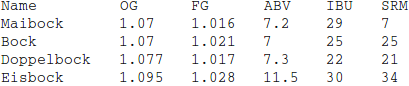
\includegraphics[scale=.5]{tabExample.png}
\end{center}
\vspace{.1in}

The first row you see is the header; your procedure does not print that row. The remaining rows are the data rows and are examples\sidenote{free test cases!} of the kind of output your procedure should produce. Each row contains a string, the name, and five doubles.
\begin{itemize}
\item  The \textit{OG} and \textit{FG}\sidenote{Original and Final Gravity} are measurements of beer taken before and after fermentation. They're always reported to three decimal places and the values fall between 1.0 and 2.0. 
\item The \textit{ABV}\sidenote{Alcohol by Volume} measures the strength of the beer. It is always reported to one decimal place. The ABV tends to fall between be between 3 and 15.
\item The \textit{IBU}\sidenote{International Bittering Units} measures the hop character and is reported with zero decimal places. The IBUs of a beer tend to be between 10 and 120.
\item The \textit{SRM}\sidenote{Standard Reference Measure} is a measure of beer color and is reported with zero decimal places. The SRM of a beer is typically between 5 and 50. 
\end{itemize}

The \textit{iomanip}\sidenote{\url{http://www.cplusplus.com/reference/iomanip/}} provides a few key manipulators for controlling how output streams print values. For this lab we're concerned with the way in which a double is printed and the general width, i.e. number of characters, values take up in genreal. The \textit{std::setprecision}\sidenote{\url{http://www.cplusplus.com/reference/iomanip/setprecision/}} manipulator lets your determine the number of decimal places printed. Be aware that this causes rounding off of values.  If you want to guarantee that the precision is exactly the number of places printed, i.e. if you want trailing zeros, then you need to use \textit{std::fixed}\sidenote{\url{http://www.cplusplus.com/reference/ios/fixed/}} from \textit{iostream}.  So, by combining std::precision and std::fixed we can make something like 1.1 print like 1.100. 


The \textit{std::setw} \sidenote{\url{http://www.cplusplus.com/reference/iomanip/setw/}} manipulator lets you specify the width of a printed value and is crucial for building a column in a table. Every column entry should print to the same number of characters. If you set the printing width to 10, then print 2.3 the stream will take care of padding the output with 7 spaces to fill the required 10 character width. By default, padding done to fill the width is done on the left. This results in right justified data. You can change this to left justification by using \textit{std::left}\sidenote{\url{http://www.cplusplus.com/reference/ios/left/}}. There's also a \textit{std::right} and a \textit{std::internal} that lets you specify an arbitrary fill point.

To build our table we want print values left-justified with the following widths: 
\begin{itemize}
\item Names should be printed 20 wide.
\item All the numerical values should be printed 8 wide.
\end{itemize}
It should be noted that the example table shown above is not necessarily printed with these width values. It was generated by Mathematica and not a C++ program.  


\end{document}

